\documentclass[aspectratio=169,12pt]{beamer}
\usepackage[utf8]{inputenc}
\usepackage{amsmath, amssymb}
\usepackage{booktabs}
\usepackage{colortbl}
\usepackage{hyperref}
\usepackage{makecell}
\usepackage{ragged2e}
\usepackage{tikz}
\usetikzlibrary{arrows.meta, positioning, shapes.geometric, calc, tikzmark, shapes.misc, fit, decorations.pathreplacing, matrix}
\usepackage{tcolorbox}
\usepackage{array}
\usepackage{listings}
\usepackage{pgfkeys}
\usepackage{adjustbox}
\usepackage[normalem]{ulem} 
\usetheme{Madrid}

% Custom colors - consolidated
\definecolor{correctgreen}{RGB}{0,150,0}
\definecolor{incorrectred}{RGB}{200,0,0}
\definecolor{counterblue}{RGB}{70,130,255}
\definecolor{highlightyellow}{RGB}{255,230,100}
\definecolor{lightblue}{RGB}{200,230,250}
\definecolor{darkblue}{RGB}{0,100,200}
\definecolor{highlightorange}{RGB}{255,200,100}

% PGF Keys for pipeline diagram configuration
\pgfkeys{
    /pipeline/.cd,
    % Stage colors
    ifcolor/.initial=lightblue,
    idcolor/.initial=lightblue,
    excolor/.initial=lightblue,
    memcolor/.initial=lightblue,
    wbcolor/.initial=lightblue,
    % Execution unit contents
    integercontent/.initial={},
    multiplycontent/.initial={},
    dividercontent/.initial={},
    % Instruction list
    instructions/.initial={},
    % Highlight colors for specific units
    highlightinteger/.initial=white,
    highlightmultiply/.initial=white,
    highlightdivider/.initial=white,
    % Individual multiply stage highlights
    highlightM1/.initial=white,
    highlightM2/.initial=white,
    highlightM3/.initial=white,
    highlightM4/.initial=white,
    % Individual divider stage highlights
    highlightD1/.initial=white,
    highlightD2/.initial=white,
    highlightD3/.initial=white,
    highlightD4/.initial=white,
    highlightD5/.initial=white,
    highlightD6/.initial=white
}

% Macro for drawing the pipeline diagram
\newcommand{\drawPipeline}[1][]{%
    \pgfkeys{/pipeline/.cd,#1}%
    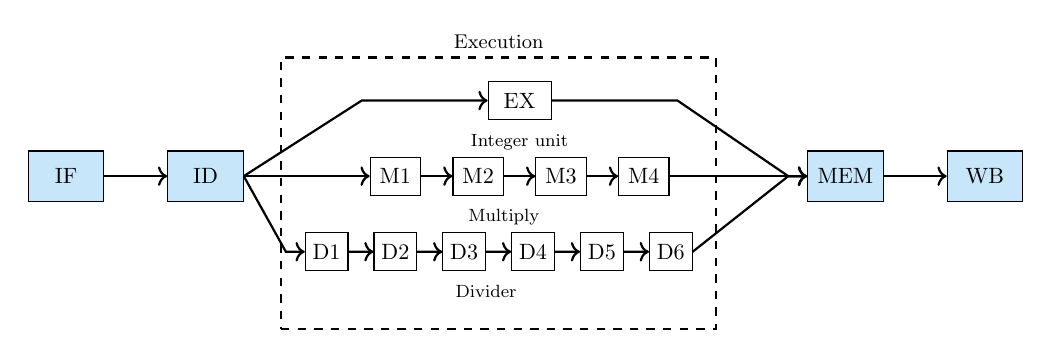
\begin{tikzpicture}[scale=0.8, transform shape]
        % Pipeline stages
        \node[draw, fill=\pgfkeysvalueof{/pipeline/ifcolor}, minimum width=1.2cm, minimum height=0.8cm] (IF) {IF};
        \node[draw, fill=\pgfkeysvalueof{/pipeline/idcolor}, minimum width=1.2cm, minimum height=0.8cm, right=of IF] (ID) {ID};
        
        % Multiply pipeline (4 stages) - each stage can be individually highlighted
        \node[draw, fill=\pgfkeysvalueof{/pipeline/highlightM1}, minimum width=0.8cm, minimum height=0.6cm, right=2cm of ID.east] (M1) {M1};
        \node[draw, fill=\pgfkeysvalueof{/pipeline/highlightM2}, minimum width=0.8cm, minimum height=0.6cm, right=0.5cm of M1] (M2) {M2};
        \node[draw, fill=\pgfkeysvalueof{/pipeline/highlightM3}, minimum width=0.8cm, minimum height=0.6cm, right=0.5cm of M2] (M3) {M3};
        \node[draw, fill=\pgfkeysvalueof{/pipeline/highlightM4}, minimum width=0.8cm, minimum height=0.6cm, right=0.5cm of M3] (M4) {M4};
        
        % Divider pipeline (multi-stage) - each stage can be individually highlighted
        \node[draw, fill=\pgfkeysvalueof{/pipeline/highlightD2}, minimum width=0.6cm, minimum height=0.6cm] (D2) at ($(M1) + (0,-1.2)$) {D2};
        \node[draw, fill=\pgfkeysvalueof{/pipeline/highlightD1}, minimum width=0.6cm, minimum height=0.6cm, left=0.4cm of D2] (D1) {D1};
        \node[draw, fill=\pgfkeysvalueof{/pipeline/highlightD3}, minimum width=0.6cm, minimum height=0.6cm, right=0.4cm of D2] (D3) {D3};
        \node[draw, fill=\pgfkeysvalueof{/pipeline/highlightD4}, minimum width=0.6cm, minimum height=0.6cm, right=0.4cm of D3] (D4) {D4};
        \node[draw, fill=\pgfkeysvalueof{/pipeline/highlightD5}, minimum width=0.6cm, minimum height=0.6cm, right=0.4cm of D4] (D5) {D5};
        \node[draw, fill=\pgfkeysvalueof{/pipeline/highlightD6}, minimum width=0.6cm, minimum height=0.6cm, right=0.4cm of D5] (D6) {D6};

        % Integer unit (single stage) - positioned between M2 and M3 horizontally, same distance above M as M is above D
        \node[draw, fill=\pgfkeysvalueof{/pipeline/highlightinteger}, minimum width=1cm, minimum height=0.6cm] (EX) at ($(M2)!0.5!(M3) + (0,1.2)$) {EX};
         
        % Labels for units
        \node[below=0.1cm of EX, font=\footnotesize] (intlabel) {Integer unit};
        \node[below=0.1cm of M2.south east, font=\footnotesize] (mullabel) {Multiply};
        \node[below=0.1cm of D3.south east, font=\footnotesize] (divlabel){Divider};

        % Execution box (drawn after units to be in background) - fits around all execution units
        \node[draw, thick, dashed, fit=(EX)(M1)(M2)(M3)(M4)(D1)(D2)(D3)(D4)(D5)(D6)(intlabel)(mullabel)(divlabel), inner sep=0.3cm] (execbox) {};
        \node[above=0 of execbox.north, anchor=south, font=\small] {Execution};
         
        % MEM and WB stages - positioned relative to execution box
        \node[draw, fill=\pgfkeysvalueof{/pipeline/memcolor}, minimum width=1.2cm, minimum height=0.8cm, right=3cm of M4.west] (MEM) {MEM};
        \node[draw, fill=\pgfkeysvalueof{/pipeline/wbcolor}, minimum width=1.2cm, minimum height=0.8cm, right=of MEM] (WB) {WB};
        
        % Connections from IF to ID
        \draw[->, thick] (IF) -- (ID);
        
        % Connections from ID to execution units - DO NOT CHANGE
        \draw[->, thick] (ID.east) -- ([xshift=-2cm]EX.west) |- (EX.west);
        \draw[->, thick] (ID.east) -- (M1.west);
        \draw[->, thick] (ID.east) -- ([xshift=-3mm]D1.west) -- (D1.west);
        
        % Connections within multiply pipeline
        \draw[->, thick] (M1) -- (M2);
        \draw[->, thick] (M2) -- (M3);
        \draw[->, thick] (M3) -- (M4);
        
        % Connections within divider pipeline
        \draw[->, thick] (D1) -- (D2);
        \draw[->, thick] (D2) -- (D3);
        \draw[->, thick] (D3) -- (D4);
        \draw[->, thick] (D4) -- (D5);
        \draw[->, thick] (D5) -- (D6);
        
        % Connections from execution units to MEM - DO NOT CHANGE
        \draw[->, thick] (EX.east) -- ([xshift=2cm]EX.east) -- ([xshift=-3mm]MEM.west) -- (MEM.west);
        \draw[->, thick] (M4.east) -- (MEM.west);
        \draw[->, thick] (D6.east) -- ([xshift=-3mm]MEM.west) -- (MEM.west);
        
        % Connection from MEM to WB
        \draw[->, thick] (MEM) -- (WB);
        
        % Add content to execution units if specified
        \pgfkeysgetvalue{/pipeline/integercontent}{\intcontent}
        \ifx\intcontent\empty\else
            \node[above=0.1cm of EX, font=\footnotesize, text=blue] {\intcontent};
        \fi
        
        \pgfkeysgetvalue{/pipeline/multiplycontent}{\mulcontent}
        \ifx\mulcontent\empty\else
            \node[above=0.1cm of M2, font=\footnotesize, text=blue] {\mulcontent};
        \fi
        
        \pgfkeysgetvalue{/pipeline/dividercontent}{\divcontent}
        \ifx\divcontent\empty\else
            \node[above=0.1cm of D3, font=\footnotesize, text=blue] {\divcontent};
        \fi
        
        % Instruction list
        \pgfkeysgetvalue{/pipeline/instructions}{\instlist}
        \ifx\instlist\empty\else
            \node[right=0.5cm of WB, align=left, font=\footnotesize] {\instlist};
        \fi
    \end{tikzpicture}%
}

% Macro for ROB diagram
\newcommand{\drawROB}[1]{%
    \begin{tikzpicture}[scale=0.8]
        \matrix (rob) [matrix of nodes,
            nodes={draw, minimum width=2cm, minimum height=0.5cm, anchor=center},
            row sep=-\pgflinewidth,
            column sep=-\pgflinewidth,
            ] {
            #1
        };
        \node[left=0.3cm of rob-1-1] {RB0};
        \node[left=0.3cm of rob-2-1] {RB1};
        \node[left=0.3cm of rob-3-1] {RB2};
        \node[left=0.3cm of rob-4-1] {RB3};
        \node[below=0.1cm of rob-4-1] {$\vdots$};
        \node[left=0.3cm of rob-5-1] {RBn};
    \end{tikzpicture}
}

% Commands for highlighting entries in detailed OOO diagrams
\newcommand{\oldentry}[1]{~#1}
\newcommand{\newentrya}[1]{\colorbox{highlightyellow}{#1}}
\newcommand{\newentryb}[1]{\colorbox{highlightorange}{#1}}
\newcommand{\newentryc}[1]{\colorbox{cyan!40}{#1}}
\newcommand{\srcentrya}[1]{\colorbox{highlightyellow!30}{#1}}
\newcommand{\srcentryb}[1]{\colorbox{highlightorange!30}{#1}}
\newcommand{\srcentryc}[1]{\colorbox{cyan!15}{#1}}

% PGF Keys for detailed OOO diagram configuration
\pgfkeys{
    /OOO/.is family, /OOO,
    default/.style = {
        % RAT registers
        R1 = {}, R2 = {}, R3 = {}, R4 = {},
        % ROB cells (2 columns x 5 rows: instruction with renamed regs, status OK/INV)
        rob01 = {}, rob02 = {},
        rob11 = {}, rob12 = {},
        rob21 = {}, rob22 = {},
        rob31 = {}, rob32 = {},
        rob41 = {}, rob42 = {},
        % RS cells
        rs1 = {~}, rs2 = {~}, rs3 = {~},
        % MOB cell
        mob1 = {~},
        % Execute cells
        exec1 = {}, exec2 = {},
        % Retire cells
        ret1 = {}, ret2 = {}, ret3 = {},
        % Instruction queue (5 rows)
        instq1 = {~}, instq2 = {~}, instq3 = {~}, instq4 = {~}, instq5 = {~}
    },
    % RAT mappings
    R1/.estore in = \prfOne,
    R2/.estore in = \prfTwo,
    R3/.estore in = \prfThree,
    R4/.estore in = \prfFour,
    % ROB cell contents
    rob01/.estore in = \robZeroOne, rob02/.estore in = \robZeroTwo,
    rob11/.estore in = \robOneOne, rob12/.estore in = \robOneTwo,
    rob21/.estore in = \robTwoOne, rob22/.estore in = \robTwoTwo,
    rob31/.estore in = \robThreeOne, rob32/.estore in = \robThreeTwo,
    rob41/.estore in = \robFourOne, rob42/.estore in = \robFourTwo,
    % RS cell contents
    rs1/.estore in = \rsOne,
    rs2/.estore in = \rsTwo,
    rs3/.estore in = \rsThree,
    % MOB cell contents
    mob1/.estore in = \mobOne,
    % Execute cell contents
    exec1/.estore in = \execOne,
    exec2/.estore in = \execTwo,
    % Retire cell contents
    ret1/.estore in = \retOne,
    ret2/.estore in = \retTwo,
    ret3/.estore in = \retThree,
    % Instruction queue (5 rows)
    instq1/.estore in = \instQOne,
    instq2/.estore in = \instQTwo,
    instq3/.estore in = \instQThree,
    instq4/.estore in = \instQFour,
    instq5/.estore in = \instQFive,
}

% Macro for drawing detailed OOO execution diagram
\newcommand{\OOODiagram}[1][]{%
    % Set defaults and process keys
    \pgfkeys{/OOO,default,#1}%
    %
    \begin{tikzpicture}[
        cell/.style={draw, minimum width=0.8cm, minimum height=0.35cm},
        smallcell/.style={draw, minimum width=0.6cm, minimum height=0.35cm},
        roundbox/.style={draw, ellipse, minimum width=3cm, minimum height=1.5cm},
        dashedbox/.style={draw, dashed, rectangle, minimum width=3cm, minimum height=1cm}
    ]
    %
    % RAT (Register Alias Table)
    \matrix[matrix of nodes,
            nodes={cell, anchor=center,
            minimum height=4mm,
            text height=1ex,
            text depth=0.25ex},
            column sep=-\pgflinewidth,
            row sep=-\pgflinewidth,
            inner sep=0pt,
            label={left:\textbf{RAT}},
            ampersand replacement=\&] (rat) {
        \scriptsize R1 \& \scriptsize \prfOne \\
        \scriptsize R2 \& \scriptsize \prfTwo \\
        \scriptsize R3 \& \scriptsize \prfThree \\
        \scriptsize R4 \& \scriptsize \prfFour \\
    };
    %
    % ROB (Reorder Buffer) - 3 columns (label, instruction with renamed regs, status)
    \matrix[matrix of nodes,
            column sep=-\pgflinewidth,
            row sep=-\pgflinewidth,
            inner sep=0pt,
            label={left:\textbf{ROB}},
            below=0.2cm of rat,
            anchor=north,
            nodes in empty cells,
            nodes={cell, align=left},
            column 1/.append style={nodes={text width=0.5cm, minimum height=4mm, text height=1ex, text depth=0.25ex}},
            column 2/.append style={nodes={text width=3.2cm, minimum height=4mm, text height=1ex, text depth=0.25ex}},
            column 3/.append style={nodes={text width=0.6cm, minimum height=4mm, text height=1ex, text depth=0.25ex}},
            ampersand replacement=\&
        ] (rob) {
    |[cell]| \scriptsize RB0 \& |[cell]| \scriptsize \robZeroOne  \& |[cell]| \scriptsize \robZeroTwo \\
    |[cell]| \scriptsize RB1 \& |[cell]| \scriptsize \robOneOne   \& |[cell]| \scriptsize \robOneTwo \\
    |[cell]| \scriptsize RB2 \& |[cell]| \scriptsize \robTwoOne   \& |[cell]| \scriptsize \robTwoTwo \\
    |[cell]| \scriptsize RB3 \& |[cell]| \scriptsize \robThreeOne \& |[cell]| \scriptsize \robThreeTwo \\
    |[cell]| \scriptsize RB4 \& |[cell]| \scriptsize \robFourOne  \& |[cell]| \scriptsize \robFourTwo \\
    };
    %
    % IDQueue - positioned right of RAT (5 rows)
    \matrix[matrix of nodes,
            row sep=-\pgflinewidth,
            column sep=-\pgflinewidth,
            inner sep=0pt,
            right=3cm of rat.north east,
            anchor=north west,
            nodes={cell, text width=3cm, align=left, minimum height=4mm, text height=1ex, text depth=0.25ex},
            label={right:\textbf{IDQ}}] (instq) {
        \scriptsize \instQOne \\
        \scriptsize \instQTwo \\
        \scriptsize \instQThree \\
        \scriptsize \instQFour \\
        \scriptsize \instQFive \\
    };
    %
    % RS (Reservation Station) - positioned below instq
    \matrix[matrix of nodes,
            row sep=-\pgflinewidth,
            inner sep=0pt,
            below=0.8cm of instq.south west,
            anchor=north west,
            nodes={cell, text width=3cm, align=left, minimum height=4mm, text height=1ex, text depth=0.25ex},
            label={above:\textbf{RS}}] (rs) {
        \scriptsize\ttfamily \rsOne \\
        \scriptsize\ttfamily \rsTwo \\
        \scriptsize\ttfamily \rsThree \\
    };
    %
    % MOB (Memory Order Buffer) - positioned right of RS
    \node[cell, right=0.5cm of rs.north east, anchor=north west, font=\scriptsize\ttfamily, text width=2.4cm, align=left] (mob) {\mobOne};
    \node[above=0.1cm of mob, font=\small] {\textbf{MOB}};
    %
    % Execute block with internal rows (no borders)
    \node[roundbox, below=0.3cm of rs.south, anchor=north] (execute) {};
    \node[anchor=west] at (execute.east) {\textbf{Execute}};
    %
    % Add internal structure to Execute (2 rows, no borders)
    \matrix[matrix of nodes,
            row sep=2pt,
            inner sep=0pt,
            at={(execute.center)},
            ampersand replacement=\&] (execMatrix) {
        |[cell/.style={minimum width=0cm, minimum height=0cm, draw=none}]| \scriptsize \execOne \\
        |[cell/.style={minimum width=0cm, minimum height=0cm, draw=none}]| \scriptsize \execTwo \\
    };
    %
    % Retire block with internal columns (no borders)
    \node[dashedbox, below=0.4cm of execute.south, anchor=north] (retire) {};
    \node[anchor=west] at (retire.east) {\textbf{Retire}};
    %
    % Add internal structure to Retire (2 columns, 2 rows, no borders)
    \matrix[matrix of nodes,
            column sep=10pt,
            row sep=2pt,
            inner sep=0pt,
            at={(retire.center)},
            ampersand replacement=\&] (retireMatrix) {
        |[cell/.style={minimum width=0cm, minimum height=0cm, draw=none}]| \scriptsize \retOne \& |[cell/.style={minimum width=0cm, minimum height=0cm, draw=none}]| \scriptsize \retTwo \\
        |[cell/.style={minimum width=0cm, minimum height=0cm, draw=none}]| \scriptsize \retThree \& |[cell/.style={minimum width=0cm, minimum height=0cm, draw=none}]| \scriptsize ~ \\
    };
    %
    \end{tikzpicture}
}

\title{Out-of-Order Execution: Part I}
\subtitle{Detailed Example}
\author{Computer Architecture 2340267}
\date{2025, Recitation \#7}

\begin{document}

\frame{\titlepage}

\begin{frame}{Execution of Instructions with Variable Execution Time}
    \begin{itemize}
        \item \textbf{Problem:} Single cycle Execution phase $\rightarrow$ The longest operation possible in the machine fixes the frequency
        \begin{itemize}
            \item Example: \textcolor{blue}{ADD/SUB=2ns, MUL=10ns, DIV=20ns} $\rightarrow$ \textcolor{red}{cc=20ns}
        \end{itemize}
        
        \item \textbf{Solution:} Implement a \textcolor{blue}{pipeline} in EXE
        \begin{itemize}
            \item Execution time of certain instructions is now variable (i.e. load with or without cache miss)
            \item More pipe stages = bigger penalty on misprediction and more data hazards (but generally an increase in CPI)
        \end{itemize}
    \end{itemize}
    
    \vspace{0.5cm}
    \centering
    \drawPipeline
\end{frame}

\begin{frame}{Pipeline Stage Progression: Multiply Unit}
    \begin{exampleblock}{Example: R2 $\leftarrow$ R3 * R3}
        The multiply operation takes 4 cycles, progressing through stages M1 $\rightarrow$ M2 $\rightarrow$ M3 $\rightarrow$ M4
    \end{exampleblock}
    \centering
    \drawPipeline
\end{frame}

\begin{frame}{Multiply Pipeline: Cycle 1}
    \centering
    \drawPipeline[
        highlightM1=highlightyellow,
        multiplycontent={R2 $\leftarrow$ R3*R3}
    ]
    \vspace{0.3cm}
    \begin{alertblock}{Stage M1}
        First stage of multiplication - operand fetch and partial product generation
    \end{alertblock}
\end{frame}

\begin{frame}{Multiply Pipeline: Cycle 2}
    \centering
    \drawPipeline[
        highlightM2=highlightyellow,
        multiplycontent={R2 $\leftarrow$ R3*R3}
    ]
    \vspace{0.3cm}
    \begin{alertblock}{Stage M2}
        Second stage - partial product accumulation
    \end{alertblock}
\end{frame}

\begin{frame}{Multiply Pipeline: Cycle 3}
    \centering
    \drawPipeline[
        highlightM3=highlightyellow,
        multiplycontent={R2 $\leftarrow$ R3*R3}
    ]
    \vspace{0.3cm}
    \begin{alertblock}{Stage M3}
        Third stage - final partial products
    \end{alertblock}
\end{frame}

\begin{frame}{Multiply Pipeline: Cycle 4}
    \centering
    \drawPipeline[
        highlightM4=correctgreen,
        multiplycontent={R2 $\leftarrow$ R3*R3}
    ]
    \vspace{0.3cm}
    \begin{alertblock}{Stage M4 - Complete}
        Final stage - result ready for writeback
    \end{alertblock}
\end{frame}

\begin{frame}{Pipeline Stage Progression: Divider Unit}
    \begin{exampleblock}{Example: R5 $\leftarrow$ R6 / R7}
        Division takes 6+ cycles, progressing through stages D1 $\rightarrow$ D2 $\rightarrow$ D3 $\rightarrow$ D4 $\rightarrow$ D5 $\rightarrow$ D6
    \end{exampleblock}
    \centering
    \drawPipeline
\end{frame}

\begin{frame}{Divider Pipeline: Cycles 1-2}
    \centering
    \drawPipeline[
        highlightD1=highlightyellow,
        highlightD2=highlightyellow,
        dividercontent={R5 $\leftarrow$ R6/R7}
    ]
    \vspace{0.3cm}
    \begin{alertblock}{Stages D1-D2}
        Initial quotient digit generation
    \end{alertblock}
\end{frame}

\begin{frame}{Divider Pipeline: Cycles 3-4}
    \centering
    \drawPipeline[
        highlightD3=highlightyellow,
        highlightD4=highlightyellow,
        dividercontent={R5 $\leftarrow$ R6/R7}
    ]
    \vspace{0.3cm}
    \begin{alertblock}{Stages D3-D4}
        Intermediate quotient refinement
    \end{alertblock}
\end{frame}

\begin{frame}{Divider Pipeline: Cycles 5-6}
    \centering
    \drawPipeline[
        highlightD5=highlightyellow,
        highlightD6=correctgreen,
        dividercontent={R5 $\leftarrow$ R6/R7}
    ]
    \vspace{0.3cm}
    \begin{alertblock}{Stages D5-D6 - Complete}
        Final quotient and remainder computation
    \end{alertblock}
\end{frame}

\begin{frame}{Example - In-Order Execution}
    \centering
    \drawPipeline[
        instructions={R1 $\leftarrow$ R1+4\\R2 $\leftarrow$ R3*R3\\R4 $\leftarrow$ R3+R4}
    ]
\end{frame}

\begin{frame}{In-Order Execution: Cycle 1}
    \centering
    \drawPipeline[
        integercontent={R1 $\leftarrow$ R1+4},
        multiplycontent={R2 $\leftarrow$ R3*R3},
        instructions={R1 $\leftarrow$ R1+4\\R2 $\leftarrow$ R3*R3\\R4 $\leftarrow$ R3+R4},
        highlightinteger=highlightyellow,
        highlightmultiply=highlightyellow
    ]
\end{frame}

\begin{frame}{In-Order Execution: Cycle 2}
    \centering
    \drawPipeline[
        integercontent={R4 $\leftarrow$ R3+R4},
        multiplycontent={R2 $\leftarrow$ R3*R3},
        instructions={R1 $\leftarrow$ R1+4\\R2 $\leftarrow$ R3*R3\\R4 $\leftarrow$ R3+R4},
        highlightinteger=highlightyellow,
        highlightmultiply=highlightyellow
    ]
    \vspace{0.5cm}
    
    \textcolor{red}{Note: R4 instruction is blocked waiting for R2 multiplication to complete!}
\end{frame}

\begin{frame}{In-Order Execution: Cycles 3-4}
    \centering
    \drawPipeline[
        multiplycontent={R2 $\leftarrow$ R3*R3},
        instructions={R1 $\leftarrow$ R1+4\\R2 $\leftarrow$ R3*R3\\R4 $\leftarrow$ R3+R4},
        highlightmultiply=highlightyellow
    ]
    \vspace{0.5cm}
    
    The multiplication continues through M2, M3, M4 stages...
\end{frame}

\begin{frame}{In-Order Execution: Final State}
    \centering
    \drawPipeline[
        integercontent={R4 $\leftarrow$ R3+R4},
        instructions={R1 $\leftarrow$ R1+4\\R2 $\leftarrow$ R3*R3\\R4 $\leftarrow$ R3+R4},
        highlightinteger=highlightyellow
    ]
    \vspace{0.5cm}
    
    Finally, R4 can execute after R2 completes
\end{frame}

\begin{frame}{Execution with Variable Time - The Problem}
    \begin{block}{Problem}
        A short operation might get "stuck" waiting for another operation of a different type to leave the Execution phase.
    \end{block}
    
    \begin{block}{Solution}
        Allow instructions of different types/pipelines to be executed \textbf{Out of Order}.
        \begin{itemize}
            \item Execute many independent instructions in parallel (in different pipelines)
            \item Improves CPI
            \item Execution must keep correctness of the code
        \end{itemize}
    \end{block}
    
    \begin{alertblock}{Note}
        If an operation gets "stuck" waiting for another operation of the same type to leave the Execution phase $\rightarrow$ \textbf{Structural Hazard} (need to add more execution units to solve).
    \end{alertblock}
\end{frame}

\begin{frame}{Out-of-Order Execution: Cycle 1}
    \centering
    \drawPipeline[
        integercontent={R1 $\leftarrow$ R1+4},
        multiplycontent={R2 $\leftarrow$ R3*R3},
        instructions={R1 $\leftarrow$ R1+4\\R2 $\leftarrow$ R3*R3\\R4 $\leftarrow$ R3+R4},
        highlightinteger=highlightyellow,
        highlightmultiply=highlightyellow
    ]
\end{frame}

\begin{frame}{Out-of-Order Execution: Cycle 2}
    \centering
    \drawPipeline[
        integercontent={R4 $\leftarrow$ R3+R4},
        multiplycontent={R2 $\leftarrow$ R3*R3},
        instructions={R1 $\leftarrow$ R1+4\\R2 $\leftarrow$ R3*R3\\R4 $\leftarrow$ R3+R4},
        highlightinteger=correctgreen,
        highlightmultiply=highlightyellow
    ]
    \vspace{0.5cm}
    
    \textcolor{correctgreen}{R4 can execute immediately - no need to wait!}
\end{frame}

\begin{frame}{CPI Limitations}
    \begin{itemize}
        \item In \textbf{in-order} machines as we've known until today, the minimum CPI achievable is 1
        \item Even with OOO execution, this limit exists as long as we only allow parallel execution in the EXE stage
    \end{itemize}
    %\begin{columns}
        %\column{0.2\textwidth}
        %\column{0.6\textwidth}
            \centering
        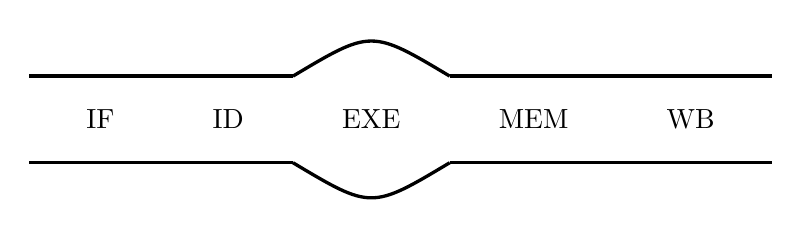
\begin{tikzpicture}[stage/.style={font=\bfseries, inner sep=1pt}]
            %--- stage labels (center line) ---
            \node (IF)  {IF};
            \node (ID)  [right=of IF]  {ID};
            \node (EXE) [right=of ID]  {EXE};
            \node (MEM) [right=of EXE] {MEM};
            \node (WB)  [right=of MEM] {WB};

            % vertical offset of the rails
            \def\dy{0.55}
            % small horizontal margin at the ends
            \def\marg{0.6}
            
            % helper points for where the bump starts/ends (midpoints around EXE)
            \coordinate (LT) at ($(ID.east)!0.5!(EXE.west)$);
            \coordinate (RT) at ($(EXE.east)!0.5!(MEM.west)$);

            %---- TOP rail: left segment, bump, right segment
            \draw[very thick] ($(IF.west)+(-\marg,\dy)$) -- ($(LT)+(0,\dy)$);
            \draw[very thick] ($(LT)+(0,\dy)$)
                .. controls ($(EXE.north)+(0,0.9)$) ..
                ($(RT)+(0,\dy)$);
            \draw[very thick] ($(RT)+(0,\dy)$) -- ($(WB.east)+(\marg,\dy)$);

            %---- BOTTOM rail: left segment, bump (down), right segment
            \draw[very thick] ($(IF.west)+(-\marg,-\dy)$) -- ($(LT)+(0,-\dy)$);
            \draw[very thick] ($(LT)+(0,-\dy)$)
                .. controls ($(EXE.south)+(0,-0.9)$) ..
                ($(RT)+(0,-\dy)$);
            \draw[very thick] ($(RT)+(0,-\dy)$) -- ($(WB.east)+(\marg,-\dy)$);
        \end{tikzpicture}
   % \end{columns}

    \begin{itemize}
        \item If we allow multiple instructions to execute in parallel in \textbf{all stages}, we can break this barrier
    \end{itemize}

    \centering
    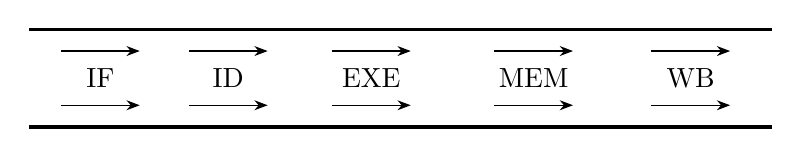
\begin{tikzpicture}[stage/.style={font=\bfseries, inner sep=1pt}]
        %--- stage labels (center line) ---
        \node (IF)  {IF};
        \node (ID)  [right=of IF]  {ID};
        \node (EXE) [right=of ID]  {EXE};
        \node (MEM) [right=of EXE] {MEM};
        \node (WB)  [right=of MEM] {WB};

        \def\dy{0.62}
        \def\dyarrowx{0.5cm}
        \def\dyarrowy{0.1cm}
        \def\marg{0.6}

        % rails
        \draw[very thick] ($(IF.west)+(-\marg,\dy)$) -- ($(WB.east)+(\marg,\dy)$);
        \draw[very thick] ($(IF.west)+(-\marg,-\dy)$) -- ($(WB.east)+(\marg,-\dy)$);
        
        \foreach \a in {IF,ID,EXE,MEM,WB}{
            \draw[-{Stealth}]
                ($(\a.north)+(-\dyarrowx,\dyarrowy)$) --
                ($(\a.north)+(\dyarrowx,\dyarrowy)$);
            \draw[-{Stealth}]
                ($(\a.south)+(-\dyarrowx,-\dyarrowy)$) --
                ($(\a.south)+(\dyarrowx,-\dyarrowy)$);
        }

    \end{tikzpicture}


    \vspace{0.5cm}
    \centering

\end{frame}

\begin{frame}{True Dependencies: RAW Hazards}
    \begin{exampleblock}{Read After Write (RAW)}
        {\ttfamily\footnotesize
        (1) ADD \textcolor{red}{R1}, R2, R3\\
        (2) ADD R5, R6, \textcolor{red}{R1}  // Must wait for \textcolor{red}{R1}
        }
    \end{exampleblock}
    
    \begin{alertblock}{Key Point}
        RAW hazards represent \textbf{true data dependencies} that cannot be eliminated—only the data flow defines program correctness.
    \end{alertblock}
\end{frame}

\begin{frame}{False Dependencies: WAR Hazards}
    \begin{exampleblock}{Write After Read (WAR)}
        {\ttfamily\footnotesize
        (1) DIV R1, R2, R3  // 40 cycles\\
        (2) ADD R5, \textcolor{red}{R6}, R1  // Waits for R1\\
        (3) ADD \textcolor{red}{R6}, R7, R8  // Could execute early!
        }
    \end{exampleblock}
    
    \begin{block}{The Problem}
        If (3) executes before (2), instruction (2) reads the \textbf{wrong} \textcolor{red}{R6} value.
    \end{block}
    
    \begin{alertblock}{Key Insight}
        WAR hazards are \textbf{artificial}—caused by register name reuse, not data flow.
    \end{alertblock}
\end{frame}

\begin{frame}{False Dependencies: WAW Hazards}
    \begin{exampleblock}{Write After Write (WAW)}
        {\ttfamily\footnotesize
        (1) DIV R1, R2, R3  // 40 cycles\\
        (2) ADD \textcolor{red}{R5}, R6, R1  // Waits for R1\\
        (3) ADD \textcolor{red}{R5}, R7, R8  // Could execute early!
        }
    \end{exampleblock}
    
    \begin{block}{The Problem}
        If (3) executes before (2), \textcolor{red}{R5} gets the \textbf{wrong} final value.
    \end{block}
    
    \begin{alertblock}{Solution Preview}
        Both WAR and WAW are \textbf{false dependencies}—register renaming eliminates them entirely.
    \end{alertblock}
\end{frame}

\begin{frame}{Register Renaming: Eliminating False Dependencies}
    \begin{block}{The Mechanism}
        \begin{itemize}
            \item \textbf{Architectural registers:} What the program sees (R0-R31)
            \item \textbf{Physical registers:} What the hardware uses (P0-P127)
            \item Dynamic mapping eliminates name conflicts
        \end{itemize}
    \end{block}
    
    \begin{exampleblock}{Renaming in Action}
        {\ttfamily\small
        \textcolor{red}{R1} $\leftarrow$ R2+R3  $\Rightarrow$  \textcolor{correctgreen}{P17} $\leftarrow$ P5+P8\\
        \textcolor{red}{R1} $\leftarrow$ R4+R5  $\Rightarrow$  \textcolor{correctgreen}{P23} $\leftarrow$ P11+P14
        }
    \end{exampleblock}
    
    \begin{alertblock}{Result}
        No WAR or WAW hazards—different physical registers for each write!
    \end{alertblock}
\end{frame}

\begin{frame}{Register Renaming - Implementation}
    We maintain two mappings:
    
    \begin{enumerate}
        \item \textbf{Architectural → Physical:} (e.g., R5→P8)
        \begin{itemize}
            \item For resolving false dependencies
            \item Saved during decode → execution transition
        \end{itemize}
        
        \item \textbf{Physical → Architectural:} (e.g., P8→R5)
        \begin{itemize}
            \item For saving the value back to the intended register
            \item Saved as part of the commit stage
        \end{itemize}
    \end{enumerate}
\end{frame}

\begin{frame}{OOO Execution Processor Architecture}
    \centering
    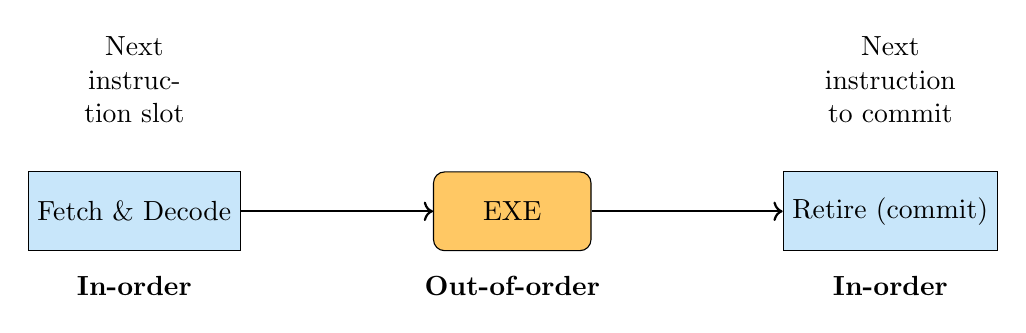
\begin{tikzpicture}[scale=1.2]
        % Stages
        \node[draw, fill=lightblue, minimum width=2cm, minimum height=1cm] (fetch) at (0,0) {Fetch \& Decode};
        \node[draw, fill=highlightorange, minimum width=2cm, minimum height=1cm, rounded corners] (exe) at (4,0) {EXE};
        \node[draw, fill=lightblue, minimum width=2cm, minimum height=1cm] (retire) at (8,0) {Retire (commit)};
        
        % Labels
        \node[below=0.2cm of fetch] {\textbf{In-order}};
        \node[below=0.2cm of exe] {\textbf{Out-of-order}};
        \node[below=0.2cm of retire] {\textbf{In-order}};
        
        % Arrows
        \draw[->, thick] (fetch) -- (exe);
        \draw[->, thick] (exe) -- (retire);
        
        % Annotations
        \node[above=0.5cm of fetch, text width=2cm, align=center] {Next instruction slot};
        \node[above=0.5cm of retire, text width=2cm, align=center] {Next instruction to commit};
    \end{tikzpicture}
    
    \vspace{0.5cm}
    Most modern processors perform fetch/decode and commit stages \textbf{in-order}, while only the execution stage is \textbf{out-of-order}.
\end{frame}

\begin{frame}{ROB (Re-Order Buffer)}
    \begin{itemize}
        \item A common implementation of Register Renaming uses ROB
        \item ROB is a buffer that receives instructions from decode stage in order
        \item The corresponding ROB entry serves as the physical register number for the instruction's destination
        \item After EXE stage, the result is written to the corresponding ROB entry
        \item Instructions commit (exit the processor) in ROB order: an instruction can only commit if the one before it has committed
    \end{itemize}
    
    \vspace{0.5cm}
    \centering
    \drawROB{
        R2/R3 \\
        R4+RB0 \\
        R3+R3 \\
        R3+RB2 \\
        {} \\
    }
\end{frame}

\begin{frame}{ROB Example - Initial State}
    \begin{columns}
        \column{0.4\textwidth}
        Instructions:
        {\ttfamily\small
        DIV R1, R2, R3\\
        ADD R2, R4, R1\\
        ADD R2, R3, R3\\
        ADD R4, R3, R2
        }
        
        \column{0.6\textwidth}
        \centering
        ROB (Cyclic Buffer):
        
        \drawROB{
            {} \\
            {} \\
            {} \\
            {} \\
            {} \\
        }
        
        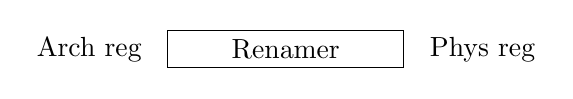
\begin{tikzpicture}
            \node[draw, minimum width=3cm] (renamer) at (0,-2) {Renamer};
            \node[left=0.2cm of renamer] {Arch reg};
            \node[right=0.2cm of renamer] {Phys reg};
        \end{tikzpicture}
    \end{columns}
\end{frame}

\begin{frame}{ROB Example - After First Instruction}
    \begin{columns}
        \column{0.4\textwidth}
        Instructions:
        {\ttfamily\small
        DIV R1, R2, R3  \checkmark\\
        ADD R2, R4, R1\\
        ADD R2, R3, R3\\
        ADD R4, R3, R2
        }

        \column{0.6\textwidth}
        \centering
        ROB:

        \drawROB{
            R2/R3 \\
            {} \\
            {} \\
            {} \\
            {} \\
        }

        \vspace{0.2cm}
        {\small R1 $\rightarrow$ RB0}
    \end{columns}
\end{frame}

\begin{frame}{ROB Example - After All Instructions}
    \begin{columns}
        \column{0.4\textwidth}
        Instructions:
        {\ttfamily\small
        DIV R1, R2, R3  \checkmark\\
        ADD R2, R4, R1  \checkmark\\
        ADD R2, R3, R3  \checkmark\\
        ADD R4, R3, R2  \checkmark
        }

        \textcolor{correctgreen}{Note: No more False Dependencies! (but RAW still exists)}

        \column{0.6\textwidth}
        \centering
        ROB:

        \drawROB{
            R2/R3 \\
            R4+RB0 \\
            R3+R3 \\
            R3+RB2 \\
            {} \\
        }

        \vspace{0.2cm}
        {\small
        R1 $\rightarrow$ RB0\\
        R2 $\rightarrow$ RB1\\
        R2 $\rightarrow$ RB2\\
        R4 $\rightarrow$ RB3
        }
    \end{columns}
\end{frame}

\begin{frame}{OOO Scheme Overview}
    \centering
    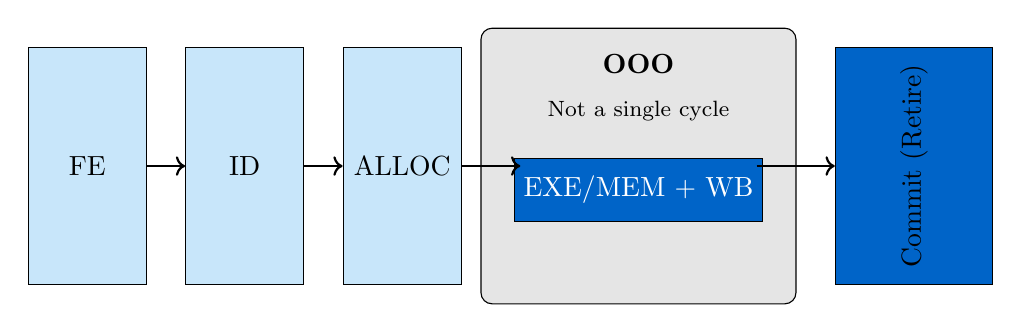
\begin{tikzpicture}[scale=1]
        % Main components
        \node[draw, fill=lightblue, minimum width=1.5cm, minimum height=3cm] (fe) at (0,0) {};
        \node at (0,0) {FE};
        
        \node[draw, fill=lightblue, minimum width=1.5cm, minimum height=3cm] (id) at (2,0) {};
        \node at (2,0) {ID};
        
        \node[draw, fill=lightblue, minimum width=1.5cm, minimum height=3cm] (alloc) at (4,0) {};
        \node at (4,0) {ALLOC};
        
        % OOO section (background box)
        \node[draw, fill=gray!20, rounded corners, minimum width=4cm, minimum height=3.5cm] (ooo) at (7,0) {};
        \node at (7,1.3) {\textbf{OOO}};
        \node at (7,0.7) {\footnotesize Not a single cycle};
        \node[draw, fill=darkblue, text=white, minimum width=3cm, minimum height=0.8cm] at (7,-0.3) {EXE/MEM + WB};
        
        \node[draw, fill=darkblue, text=white, minimum width=2cm, minimum height=3cm] (commit) at (10.5,0) {};
        \node[rotate=90] at (10.5,0) {Commit (Retire)};
        
        % Arrows
        \draw[->, thick] (fe) -- (id);
        \draw[->, thick] (id) -- (alloc);
        \draw[->, thick] (alloc) -- (5.5,0);
        \draw[->, thick] (8.5,0) -- (commit);
    \end{tikzpicture}
\end{frame}

\begin{frame}{Summary: Out-of-Order Execution}
    \textbf{The Journey:}
    \begin{enumerate}
        \item \textbf{Problem:} Long-latency operations stall the pipeline
        \item \textbf{Solution:} Execute independent instructions out of order
        \item \textbf{Challenge:} False dependencies (WAR, WAW)
        \item \textbf{Solution:} Register renaming with ROB
    \end{enumerate}

    \vspace{0.5cm}
    \textbf{Modern Processor Pipeline:}
    \begin{itemize}
        \item \textbf{Front-end:} In-order fetch and decode
        \item \textbf{Execution:} Out-of-order with multiple units
        \item \textbf{Back-end:} In-order commit (retirement)
    \end{itemize}

    \vspace{0.5cm}
    \textbf{Bottom Line:} OOO execution dramatically improves IPC by hiding latencies and maximizing parallelism.
\end{frame}

\begin{frame}{Historical Note: IBM System/360 Model 91 (1966)}
    \begin{columns}
        \column{0.4\textwidth}
        \includegraphics[width=\textwidth]{figures/ibm360m91.jpg}

        \vspace{0.2cm}
        \scriptsize Photo: NASA Goddard Space Flight Center
        {
            \fontsize{4}{5}\selectfont
            By Bundesarchiv, B 145 Bild-F038812-0014 / Schaack, Lothar /
            \href{https://commons.wikimedia.org/w/index.php?curid=5455799}{CC-BY-SA 3.0}
        }

        \column{0.6\textwidth}
        \begin{itemize}
            \item \textbf{First IBM computer} with out-of-order execution
            \item Developed by Robert Tomasulo at IBM
            \item Introduced the \textbf{Tomasulo Algorithm}:
            \begin{itemize}
                \footnotesize
                \item Register renaming via reservation stations
                \item Dynamic scheduling
                \item Common Data Bus (CDB) for results
            \end{itemize}
            \item \textbf{Performance:} 16.6 MFLOPS peak
            \item \textbf{Cost:} \$6-7 million (1966 dollars)
        \end{itemize}
    \end{columns}

    \vspace{0.3cm}
    \begin{alertblock}{Legacy}
        The Tomasulo algorithm's concepts remain fundamental to modern processors—every high-performance CPU today uses variations of these techniques.
    \end{alertblock}
\end{frame}

\begin{frame}{Detailed OOO Execution Example}
    \begin{block}{Goal}
        Trace a complete out-of-order execution cycle-by-cycle, showing:
        \begin{itemize}
            \item Register Alias Table (RAT) updates
            \item Reorder Buffer (ROB) allocation
            \item Reservation Station (RS) scheduling
            \item Memory Order Buffer (MOB) management
            \item Execute and Retire stages
        \end{itemize}
    \end{block}

    \begin{block}{Key Structures}
        \begin{itemize}
            \item \textbf{RAT:} Maps architectural registers to physical registers (ROB entries)
            \item \textbf{ROB:} Circular buffer maintaining program order (RB0-RB4)
            \item \textbf{IDQ:} Instruction Decode Queue holding fetched instructions
            \item \textbf{RS:} Holds decoded instructions waiting for operands
            \item \textbf{MOB:} Manages memory operations in order
        \end{itemize}
    \end{block}
\end{frame}

\begin{frame}{Example: Out-of-Order Execution}
    \textbf{Question:} How many cycles will it take to execute the following program using out-of-order execution?

    \textit{Assume all instructions have already been decoded and are in the IDQ.}

    \vspace{0.4cm}
    \begin{columns}[T]
        \begin{column}{0.5\textwidth}
            \textbf{Program:}

            {\ttfamily\small
            \begin{tabular}{ll}
            (1) & DIV R2, R4, R3 \\
            (2) & LD R3, R4(50) \\
            (3) & DIV R1, R2, R3 \\
            (4) & ADD R2, R4, R3 \\
            (5) & SUB R3, R2, R3 \\
            \end{tabular}
            }
        \end{column}
        \begin{column}{0.45\textwidth}
            \textbf{Latencies:}

            \begin{itemize}
                \item \textbf{DIV:} 4 cycles
                \item \textbf{LD:} 2 cycles
                \item \textbf{ADD/SUB:} 1 cycle
            \end{itemize}
        \end{column}
    \end{columns}

    \vspace{0.4cm}
    \begin{alertblock}{Observation}
        Instructions (1) and (2) are independent and can execute in parallel. Instruction (3) depends on both (1) and (2).
    \end{alertblock}
\end{frame}

\begin{frame}{Notation for Cycle-by-Cycle Walkthrough}
    \begin{block}{Execution Status Notation}
        In the \textbf{Execute} section, we show operations currently being executed with their \textbf{remaining cycle count} in brackets.

        \vspace{0.3cm}
        \textbf{Example:} RB0$\leftarrow$R4/R3 [3]
        \begin{itemize}
            \item This means ROB entry RB0 is executing the DIV operation R4/R3
            \item There are \textbf{3 cycles remaining} until this operation completes
            \item Next cycle, this will show [2], then [1], then complete
        \end{itemize}
    \end{block}

    \vspace{0.2cm}
    \begin{exampleblock}{Operation Latencies (Reminder)}
        \begin{itemize}
            \item DIV: 4 cycles → shows [4], [3], [2], [1]
            \item LD: 2 cycles → shows [2], [1]
            \item ADD/SUB: 1 cycle → shows [1]
        \end{itemize}
    \end{exampleblock}
\end{frame}

\begin{frame}{Cycle 1: Decode}
    \centering
    \OOODiagram[
        R1={}, R2={\newentrya{RB0}}, R3={}, R4={},
        rob01={\newentrya{R2$\leftarrow$R4/R3}}, rob02={\newentrya{INV}},
        rs1={\newentrya{RB0$\leftarrow$R4/R3}},
        instq1={SUB R3,R2,R3}, instq2={ADD R2,R4,R3}, instq3={DIV R1,R2,R3}, instq4={LD R3,R4(50)}, instq5={\newentrya{\sout{DIV R2,R4,R3}}}
    ]

    \vspace{0.3cm}
    \begin{tikzpicture}[remember picture, overlay]
        \node[anchor=south west, text width=6cm, font=\small, yshift=0.5cm] at (current page.south west) {
            \begin{block}{What's Happening}
                First instruction (DIV R2,R4,R3) is decoded. RAT maps R2→RB0, ROB allocates RB0, and RS receives the operation with operands ready.
            \end{block}
        };
    \end{tikzpicture}
\end{frame}

\begin{frame}{Cycle 2: Execute}
    \centering
    \OOODiagram[
        R1={}, R2={\oldentry{RB0}}, R3={}, R4={},
        rob01={\oldentry{R2$\leftarrow$R4/R3}}, rob02={\oldentry{INV}},
        rs1={\srcentrya{\sout{RB0$\leftarrow$R4/R3}}},
        exec1={\newentrya{RB0$\leftarrow$R4/R3 [4]}},
        instq1={SUB R3,R2,R3}, instq2={ADD R2,R4,R3}, instq3={DIV R1,R2,R3}, instq4={LD R3,R4(50)}, instq5={~}
    ]

    \vspace{0.3cm}
    \begin{tikzpicture}[remember picture, overlay]
        \node[anchor=south west, text width=6cm, font=\small, yshift=0.5cm] at (current page.south west) {
            \begin{block}{What's Happening}
                RB0 (DIV) dispatched from RS to execution unit. DIV takes 4 cycles, shown as [4].
            \end{block}
        };
    \end{tikzpicture}
\end{frame}

\begin{frame}{Cycle 2: Decode}
    \centering
    \OOODiagram[
        R1={}, R2={\oldentry{RB0}}, R3={\newentrya{RB1}}, R4={},
        rob01={\oldentry{R2$\leftarrow$R4/R3}}, rob02={\oldentry{INV}},
        rob11={\newentrya{R3$\leftarrow$LD R4(50)}}, rob12={\newentrya{INV}},
        rs1={\newentrya{MOB$\leftarrow$R4+50}},
        exec1={\oldentry{RB0$\leftarrow$R4/R3 [4]}},
        mob1={\newentrya{RB1$\leftarrow$MEM(?) [W]}},
        instq1={SUB R3,R2,R3}, instq2={ADD R2,R4,R3}, instq3={DIV R1,R2,R3}, instq4={\srcentrya{\sout{LD R3,R4(50)}}}, instq5={~}
    ]

    \vspace{0.3cm}
    \begin{tikzpicture}[remember picture, overlay]
        \node[anchor=south west, text width=6cm, font=\small, yshift=0.5cm] at (current page.south west) {
            \begin{block}{What's Happening}
                LD decoded: RAT maps R3→RB1, ROB allocates RB1. MOB entry created with [W] - waiting for address R4+50 to be computed.
            \end{block}
        };
    \end{tikzpicture}
\end{frame}

\begin{frame}{Cycle 3: Execute}
    \centering
    \OOODiagram[
        R1={}, R2={\oldentry{RB0}}, R3={\oldentry{RB1}}, R4={},
        rob01={\oldentry{R2$\leftarrow$R4/R3}}, rob02={\oldentry{INV}},
        rob11={\oldentry{R3$\leftarrow$LD R4(50)}}, rob12={\oldentry{INV}},
        exec1={\newentrya{RB0$\leftarrow$R4/R3 [3]}},
        exec2={\newentryb{MOB$\leftarrow$R4+50}},
        mob1={\oldentry{RB1$\leftarrow$MEM(?) [W]}},
        instq1={SUB R3,R2,R3}, instq2={ADD R2,R4,R3}, instq3={DIV R1,R2,R3}, instq4={~}, instq5={~}
    ]

    \vspace{0.3cm}
    \begin{tikzpicture}[remember picture, overlay]
        \node[anchor=south west, text width=6cm, font=\small, yshift=0.5cm] at (current page.south west) {
            \begin{block}{What's Happening}
                RB0 continues executing [4→3]. Address R4+50 computed (ADD takes 1 cycle). MOB still waiting [W] for address to complete.
            \end{block}
        };
    \end{tikzpicture}
\end{frame}

\begin{frame}{Cycle 3: Decode}
    \centering
    \OOODiagram[
        R1={\newentrya{RB2}}, R2={\oldentry{RB0}}, R3={\oldentry{RB1}}, R4={},
        rob01={\oldentry{R2$\leftarrow$R4/R3}}, rob02={\oldentry{INV}},
        rob11={\oldentry{R3$\leftarrow$LD R4(50)}}, rob12={\oldentry{INV}},
        rob21={\newentrya{R1$\leftarrow$RB0/RB1}}, rob22={\newentrya{INV}},
        rs2={\newentrya{RB2$\leftarrow$\textcolor{red}{RB0}/\textcolor{red}{RB1}}},
        exec1={\oldentry{RB0$\leftarrow$R4/R3 [3]}},
        exec2={\oldentry{MOB$\leftarrow$R4+50}},
        mob1={\oldentry{RB1$\leftarrow$MEM(?) [W]}},
        instq1={SUB R3,R2,R3}, instq2={ADD R2,R4,R3}, instq3={\srcentrya{\sout{DIV R1,R2,R3}}}, instq4={~}, instq5={~}
    ]

    \vspace{0.3cm}
    \begin{tikzpicture}[remember picture, overlay]
        \node[anchor=south west, text width=6cm, font=\small, yshift=0.5cm] at (current page.south west) {
            \begin{block}{What's Happening}
                DIV R1 decoded - depends on RB0 and RB1, goes to RS but can't execute yet. LD now dispatched from MOB with [2] cycles. RB0 continues at [3].
            \end{block}
        };
    \end{tikzpicture}
\end{frame}

\begin{frame}{Cycle 4: Execute}
    \centering
    \OOODiagram[
        R1={\oldentry{RB2}}, R2={\oldentry{RB3}}, R3={\oldentry{RB1}}, R4={},
        rob01={\oldentry{R2$\leftarrow$R4/R3}}, rob02={\oldentry{INV}},
        rob11={\oldentry{R3$\leftarrow$LD R4(50)}}, rob12={\oldentry{INV}},
        rob21={\oldentry{R1$\leftarrow$RB0/RB1}}, rob22={\oldentry{INV}},
        rob31={\oldentry{R2$\leftarrow$R4+RB1}}, rob32={\oldentry{INV}},
        rs2={\oldentry{RB2$\leftarrow$\textcolor{red}{RB0}/\textcolor{red}{RB1} [W]}},
        rs3={\oldentry{RB3$\leftarrow$R4+\textcolor{red}{RB1} [W]}},
        exec1={\newentrya{RB0$\leftarrow$R4/R3 [2]}},
        exec2={\srcentryb{\sout{MOB$\leftarrow$R4+50}}},
        mob1={\newentryb{RB1$\leftarrow$R4(50) [2]}},
        instq1={SUB R3,R2,R3}, instq2={ADD R2,R4,R3}, instq3={~}, instq4={~}, instq5={~}
    ]

    \vspace{0.3cm}
    \begin{tikzpicture}[remember picture, overlay]
        \node[anchor=south west, text width=6cm, font=\small, yshift=0.5cm] at (current page.south west) {
            \begin{block}{What's Happening}
                RB0 (DIV) at [3]. RB1 (LD) completes - last cycle [1]. ROB will be marked OK after this cycle.
            \end{block}
        };
    \end{tikzpicture}
\end{frame}

\begin{frame}{Cycle 4: Decode}
    \centering
    \OOODiagram[
        R1={\oldentry{RB2}}, R2={\newentrya{RB3}}, R3={\oldentry{RB1}}, R4={},
        rob01={\oldentry{R2$\leftarrow$R4/R3}}, rob02={\oldentry{INV}},
        rob11={\oldentry{R3$\leftarrow$LD R4(50)}}, rob12={\oldentry{INV}},
        rob21={\oldentry{R1$\leftarrow$RB0/RB1}}, rob22={\oldentry{INV}},
        rob31={\newentrya{R2$\leftarrow$R4+RB1}}, rob32={\newentrya{INV}},
        rs2={\oldentry{RB2$\leftarrow$\textcolor{red}{RB0}/\textcolor{red}{RB1} [W]}},
        rs3={\newentrya{RB3$\leftarrow$R4+\textcolor{red}{RB1} [W]}},
        exec1={\oldentry{RB0$\leftarrow$R4/R3 [2]}},
        mob1={\oldentry{RB1$\leftarrow$R4(50) [2]}},
        instq1={SUB R3,R2,R3}, instq2={\srcentrya{\sout{ADD R2,R4,R3}}}, instq3={~}, instq4={~}, instq5={~}
    ]

    \vspace{0.3cm}
    \begin{tikzpicture}[remember picture, overlay]
        \node[anchor=south west, text width=6cm, font=\small, yshift=0.5cm] at (current page.south west) {
            \begin{block}{What's Happening}
                ADD decoded: RAT maps R2→RB3 (old RB0 still in ROB). RS entry waits for RB1. RB1 completes, ROB marked OK. RB0 at [3].
            \end{block}
        };
    \end{tikzpicture}
\end{frame}

\begin{frame}{Cycle 5: Execute}
    \centering
    \OOODiagram[
        R1={\oldentry{RB2}}, R2={\oldentry{RB3}}, R3={\oldentry{RB1}}, R4={},
        rob01={\oldentry{R2$\leftarrow$R4/R3}}, rob02={\oldentry{INV}},
        rob11={\oldentry{R3$\leftarrow$LD R4(50)}}, rob12={\oldentry{INV}},
        rob21={\oldentry{R1$\leftarrow$RB0/RB1}}, rob22={\oldentry{INV}},
        rob31={\oldentry{R2$\leftarrow$R4+RB1}}, rob32={\oldentry{INV}},
        rs2={\oldentry{RB2$\leftarrow$\textcolor{red}{RB0}/\textcolor{red}{RB1} [W]}},
        rs3={\oldentry{RB3$\leftarrow$R4+\textcolor{red}{RB1} [W]}},
        exec1={\newentrya{RB0$\leftarrow$R4/R3 [1]}},
        mob1={\newentrya{RB1$\leftarrow$R4(50) [1]}},
        instq1={SUB R3,R2,R3}, instq2={~}, instq3={~}, instq4={~}, instq5={~}
    ]

    \vspace{0.3cm}
    \begin{tikzpicture}[remember picture, overlay]
        \node[anchor=south west, text width=6cm, font=\small, yshift=0.5cm] at (current page.south west) {
            \begin{block}{What's Happening}
                RB0 (DIV) at [1]. RS blocked: RB2 waiting [W] on RB0 and RB1 dependencies, cannot dispatch. MOB at [1]. Retirement stalled waiting for RB0 to complete.
            \end{block}
        };
    \end{tikzpicture}
\end{frame}

\begin{frame}{Cycle 5: Decode}
    \centering
    \OOODiagram[
        R1={\oldentry{RB2}}, R2={\oldentry{RB3}}, R3={\newentrya{RB4}}, R4={},
        rob01={\oldentry{R2$\leftarrow$R4/R3}}, rob02={\oldentry{INV}},
        rob11={\oldentry{R3$\leftarrow$LD R4(50)}}, rob12={\oldentry{INV}},
        rob21={\oldentry{R1$\leftarrow$RB0/RB1}}, rob22={\oldentry{INV}},
        rob31={\oldentry{R2$\leftarrow$R4+RB1}}, rob32={\oldentry{INV}},
        rob41={\newentrya{R3$\leftarrow$RB3-RB1}}, rob42={\newentrya{INV}},
        rs1={\newentrya{RB4$\leftarrow$\textcolor{red}{RB3}-\textcolor{red}{RB1} [W]}},
        rs2={\oldentry{RB2$\leftarrow$\textcolor{red}{RB0}/\textcolor{red}{RB1} [W]}},
        rs3={\oldentry{RB3$\leftarrow$R4+\textcolor{red}{RB1} [W]}},
        exec1={\oldentry{RB0$\leftarrow$R4/R3 [1]}},
        mob1={\oldentry{RB1$\leftarrow$R4(50) [1]}},
        ret1={\oldentry{R3$\leftarrow$RB1}},
        instq1={\srcentrya{\sout{SUB R3,R2,R3}}}, instq2={~}, instq3={~}, instq4={~}, instq5={~}
    ]

    \vspace{0.3cm}
    \begin{tikzpicture}[remember picture, overlay]
        \node[anchor=south west, text width=6cm, font=\small, yshift=0.5cm] at (current page.south west) {
            \begin{block}{What's Happening}
                SUB decoded, creates RB4 in ROB with dependencies on RB3 and RB1. RB4 enters RS waiting for RB3. RB3 dispatched to execute. RB0 at [2].
            \end{block}
        };
    \end{tikzpicture}
\end{frame}

\begin{frame}{Cycle 6: Execution Completes}
    \centering
    \OOODiagram[
        R1={\oldentry{RB2}}, R2={\oldentry{RB3}}, R3={\oldentry{RB4}}, R4={},
        rob01={\oldentry{R2$\leftarrow$R4/R3}}, rob02={\newentryb{OK}},
        rob11={\oldentry{R3$\leftarrow$LD R4(50)}}, rob12={\newentrya{OK}},
        rob21={\oldentry{R1$\leftarrow$RB0/RB1}}, rob22={\oldentry{INV}},
        rob31={\oldentry{R2$\leftarrow$R4+RB1}}, rob32={\oldentry{INV}},
        rob41={\oldentry{R3$\leftarrow$RB3-RB1}}, rob42={\oldentry{INV}},
        rs1={\oldentry{RB4$\leftarrow$\textcolor{red}{RB3}-\newentrya{RB1} [W]}},
        rs2={\oldentry{RB2$\leftarrow$\newentryb{RB0}/\newentrya{RB1}}},
        rs3={\oldentry{RB3$\leftarrow$R4+\newentrya{RB1}}},
        exec1={\srcentryb{\sout{RB0$\leftarrow$R4/R3}}},
        mob1={\srcentrya{\sout{RB1$\leftarrow$R4(50)}}},
        instq1={~}, instq2={~}, instq3={~}, instq4={~}, instq5={~}
    ]

    \vspace{0.3cm}
    \begin{tikzpicture}[remember picture, overlay]
        \node[anchor=south west, text width=6cm, font=\small, yshift=0.5cm] at (current page.south west) {
            \begin{block}{What's Happening}
                RB0 (DIV) and RB1 (LD) complete, marked OK. Forwarding: RB2 and RB3 in RS now unblocked, ready to dispatch. RB4 still waiting [W] on RB3.
            \end{block}
        };
    \end{tikzpicture}
\end{frame}

\begin{frame}{Cycle 6: Execute}
    \centering
    \OOODiagram[
        R1={\oldentry{RB2}}, R2={\oldentry{RB3}}, R3={\oldentry{RB4}}, R4={},
        rob01={\oldentry{R2$\leftarrow$R4/R3}}, rob02={\oldentry{OK}},
        rob11={\oldentry{R3$\leftarrow$LD R4(50)}}, rob12={\oldentry{OK}},
        rob21={\oldentry{R1$\leftarrow$RB0/RB1}}, rob22={\oldentry{INV}},
        rob31={\oldentry{R2$\leftarrow$R4+RB1}}, rob32={\oldentry{INV}},
        rob41={\oldentry{R3$\leftarrow$RB3-RB1}}, rob42={\oldentry{INV}},
        rs1={\oldentry{RB4$\leftarrow$\textcolor{red}{RB3}-RB1 [W]}},
        rs2={\srcentrya{\sout{RB2$\leftarrow$RB0/RB1}}},
        rs3={\srcentryb{\sout{RB3$\leftarrow$R4+RB1}}},
        exec1={\newentrya{RB2$\leftarrow$RB0/RB1 [4]}},
        exec2={\newentryb{RB3$\leftarrow$R4+RB1 [1]}},
        instq1={~}, instq2={~}, instq3={~}, instq4={~}, instq5={~}
    ]

    \vspace{0.3cm}
    \begin{tikzpicture}[remember picture, overlay]
        \node[anchor=south west, text width=6cm, font=\small, yshift=0.5cm] at (current page.south west) {
            \begin{block}{What's Happening}
                RB2 (DIV) and RB3 (ADD) dispatch from RS and start executing [4] and [1]. RB4 still waiting [W] on RB3. No retirement yet.
            \end{block}
        };
    \end{tikzpicture}
\end{frame}

\begin{frame}{Cycle 7: Retire}
    \centering
    \OOODiagram[
        R1={\oldentry{RB2}}, R2={\oldentry{RB3}}, R3={\oldentry{RB4}}, R4={},
        rob01={\srcentrya{\sout{R2$\leftarrow$R4/R3}}}, rob02={\srcentrya{\sout{OK}}},
        rob11={\srcentryb{\sout{R3$\leftarrow$LD R4(50)}}}, rob12={\srcentryb{\sout{OK}}},
        rob21={\oldentry{R1$\leftarrow$RB0/RB1}}, rob22={\oldentry{INV}},
        rob31={\oldentry{R2$\leftarrow$R4+RB1}}, rob32={\oldentry{INV}},
        rob41={\oldentry{R3$\leftarrow$RB3-RB1}}, rob42={\oldentry{INV}},
        rs1={\oldentry{RB4$\leftarrow$\textcolor{red}{RB3}-RB1 [W]}},
        exec1={\oldentry{RB2$\leftarrow$RB0/RB1 [4]}},
        exec2={\oldentry{RB3$\leftarrow$R4+RB1 [1]}},
        ret1={\newentrya{R2$\leftarrow$RB0}},
        ret2={\newentryb{R3$\leftarrow$RB1}},
        instq1={~}, instq2={~}, instq3={~}, instq4={~}, instq5={~}
    ]

    \vspace{0.3cm}
    \begin{tikzpicture}[remember picture, overlay]
        \node[anchor=south west, text width=6cm, font=\small, yshift=0.5cm] at (current page.south west) {
            \begin{block}{What's Happening}
                RB0 and RB1 retire, committing R2 and R3. ROB entries freed. RB2 continues [4], RB3 continues [1].
            \end{block}
        };
    \end{tikzpicture}
\end{frame}

\begin{frame}{Cycle 7: Execution Completes}
    \centering
    \OOODiagram[
        R1={\oldentry{RB2}}, R2={\oldentry{RB3}}, R3={\oldentry{RB4}}, R4={},
        rob21={\oldentry{R1$\leftarrow$RB0/RB1}}, rob22={\oldentry{INV}},
        rob31={\oldentry{R2$\leftarrow$R4+RB1}}, rob32={\newentrya{OK}},
        rob41={\oldentry{R3$\leftarrow$RB3-RB1}}, rob42={\oldentry{INV}},
        rs1={\oldentry{RB4$\leftarrow$\newentrya{RB3}-RB1}},
        exec1={\oldentry{RB2$\leftarrow$RB0/RB1 [4]}},
        exec2={\srcentrya{\sout{RB3$\leftarrow$R4+RB1}}},
        instq1={~}, instq2={~}, instq3={~}, instq4={~}, instq5={~}
    ]

    \vspace{0.3cm}
    \begin{tikzpicture}[remember picture, overlay]
        \node[anchor=south west, text width=6cm, font=\small, yshift=0.5cm] at (current page.south west) {
            \begin{block}{What's Happening}
                RB3 (ADD) completes execution. Result forwarded to RB4 in RS - RB3 dependency resolved, no longer waiting [W].
            \end{block}
        };
    \end{tikzpicture}
\end{frame}

\begin{frame}{Cycle 7: Execute}
    \centering
    \OOODiagram[
        R1={\oldentry{RB2}}, R2={\oldentry{RB3}}, R3={\oldentry{RB4}}, R4={},
        rob21={\oldentry{R1$\leftarrow$RB0/RB1}}, rob22={\oldentry{INV}},
        rob31={\oldentry{R2$\leftarrow$R4+RB1}}, rob32={\oldentry{OK}},
        rob41={\oldentry{R3$\leftarrow$RB3-RB1}}, rob42={\oldentry{INV}},
        rs1={\srcentryb{\sout{RB4$\leftarrow$RB3-RB1}}},
        exec1={\newentrya{RB2$\leftarrow$RB0/RB1 [3]}},
        exec2={\newentryb{RB4$\leftarrow$RB3-RB1 [1]}},
        instq1={~}, instq2={~}, instq3={~}, instq4={~}, instq5={~}
    ]

    \vspace{0.3cm}
    \begin{tikzpicture}[remember picture, overlay]
        \node[anchor=south west, text width=6cm, font=\small, yshift=0.5cm] at (current page.south west) {
            \begin{block}{What's Happening}
                RB2 (DIV) continues [3]. RB4 (SUB) dispatches from RS and starts executing [1]. Nothing to decode.
            \end{block}
        };
    \end{tikzpicture}
\end{frame}

\begin{frame}{Cycle 8: Retire}
    \centering
    \OOODiagram[
        R1={\oldentry{RB2}}, R2={\oldentry{RB3}}, R3={\oldentry{RB4}}, R4={},
        rob21={\srcentrya{R1$\leftarrow$RB0/RB1}}, rob22={\srcentrya{INV}},
        rob31={\oldentry{R2$\leftarrow$R4+RB1}}, rob32={\oldentry{OK}},
        rob41={\oldentry{R3$\leftarrow$RB3-RB1}}, rob42={\oldentry{INV}},
        exec1={\oldentry{RB2$\leftarrow$RB0/RB1 [3]}},
        exec2={\oldentry{RB4$\leftarrow$RB3-RB1 [1]}},
        instq1={~}, instq2={~}, instq3={~}, instq4={~}, instq5={~}
    ]

    \vspace{0.3cm}
    \begin{tikzpicture}[remember picture, overlay]
        \node[anchor=south west, text width=6cm, font=\small, yshift=0.5cm] at (current page.south west) {
            \begin{block}{What's Happening}
                No retirement can take place. RB2 is at the head of ROB but still INV (not complete). Despite RB3 being OK and ready, it cannot retire - must retire in-order.
            \end{block}
        };
    \end{tikzpicture}
\end{frame}

\begin{frame}{Cycle 8: Execute}
    \centering
    \OOODiagram[
        R1={\oldentry{RB2}}, R2={\oldentry{RB3}}, R3={\oldentry{RB4}}, R4={},
        rob21={\oldentry{R1$\leftarrow$RB0/RB1}}, rob22={\oldentry{INV}},
        rob31={\oldentry{R2$\leftarrow$R4+RB1}}, rob32={\oldentry{OK}},
        rob41={\oldentry{R3$\leftarrow$RB3-RB1}}, rob42={\newentryb{OK}},
        exec1={\newentrya{RB2$\leftarrow$RB0/RB1 [2]}},
        exec2={\srcentryb{\sout{RB4$\leftarrow$RB3-RB1}}},
        instq1={~}, instq2={~}, instq3={~}, instq4={~}, instq5={~}
    ]

    \vspace{0.3cm}
    \begin{tikzpicture}[remember picture, overlay]
        \node[anchor=south west, text width=6cm, font=\small, yshift=0.5cm] at (current page.south west) {
            \begin{block}{What's Happening}
                RB2 (DIV) continues [2]. RB4 (SUB) completes execution, writes result to ROB. Nothing to decode.
            \end{block}
        };
    \end{tikzpicture}
\end{frame}

\begin{frame}{Cycle 9: Retire}
    \centering
    \OOODiagram[
        R1={\oldentry{RB2}}, R2={\oldentry{RB3}}, R3={\oldentry{RB4}}, R4={},
        rob21={\srcentrya{R1$\leftarrow$RB0/RB1}}, rob22={\srcentrya{INV}},
        rob31={\oldentry{R2$\leftarrow$R4+RB1}}, rob32={\oldentry{OK}},
        rob41={\oldentry{R3$\leftarrow$RB3-RB1}}, rob42={\oldentry{OK}},
        exec1={\oldentry{RB2$\leftarrow$RB0/RB1 [2]}},
        instq1={~}, instq2={~}, instq3={~}, instq4={~}, instq5={~}
    ]

    \vspace{0.3cm}
    \begin{tikzpicture}[remember picture, overlay]
        \node[anchor=south west, text width=6cm, font=\small, yshift=0.5cm] at (current page.south west) {
            \begin{block}{What's Happening}
                Again, no commit. RB2 still INV. Despite RB3 and RB4 being OK, must commit in-order.
            \end{block}
        };
    \end{tikzpicture}
\end{frame}

\begin{frame}{Cycle 9: Execute}
    \centering
    \OOODiagram[
        R1={\oldentry{RB2}}, R2={\oldentry{RB3}}, R3={\oldentry{RB4}}, R4={},
        rob21={\oldentry{R1$\leftarrow$RB0/RB1}}, rob22={\oldentry{INV}},
        rob31={\oldentry{R2$\leftarrow$R4+RB1}}, rob32={\oldentry{OK}},
        rob41={\oldentry{R3$\leftarrow$RB3-RB1}}, rob42={\oldentry{OK}},
        exec1={\newentrya{RB2$\leftarrow$RB0/RB1 [1]}},
        instq1={~}, instq2={~}, instq3={~}, instq4={~}, instq5={~}
    ]

    \vspace{0.3cm}
    \begin{tikzpicture}[remember picture, overlay]
        \node[anchor=south west, text width=6cm, font=\small, yshift=0.5cm] at (current page.south west) {
            \begin{block}{What's Happening}
                RB2 (DIV) continues [1]. Nothing to decode.
            \end{block}
        };
    \end{tikzpicture}
\end{frame}

\begin{frame}{Cycle 10: Retire}
    \centering
    \OOODiagram[
        R1={\oldentry{RB2}}, R2={\oldentry{RB3}}, R3={\oldentry{RB4}}, R4={},
        rob21={\srcentrya{R1$\leftarrow$RB0/RB1}}, rob22={\srcentrya{INV}},
        rob31={\oldentry{R2$\leftarrow$R4+RB1}}, rob32={\oldentry{OK}},
        rob41={\oldentry{R3$\leftarrow$RB3-RB1}}, rob42={\oldentry{OK}},
        exec1={\oldentry{RB2$\leftarrow$RB0/RB1 [1]}},
        instq1={~}, instq2={~}, instq3={~}, instq4={~}, instq5={~}
    ]

    \vspace{0.3cm}
    \begin{tikzpicture}[remember picture, overlay]
        \node[anchor=south west, text width=6cm, font=\small, yshift=0.5cm] at (current page.south west) {
            \begin{block}{What's Happening}
                Again, nothing to retire. RB2 still INV. Must retire in-order.
            \end{block}
        };
    \end{tikzpicture}
\end{frame}

\begin{frame}{Cycle 10: Execute}
    \centering
    \OOODiagram[
        R1={\oldentry{RB2}}, R2={\oldentry{RB3}}, R3={\oldentry{RB4}}, R4={},
        rob21={\oldentry{R1$\leftarrow$RB0/RB1}}, rob22={\newentrya{OK}},
        rob31={\oldentry{R2$\leftarrow$R4+RB1}}, rob32={\oldentry{OK}},
        rob41={\oldentry{R3$\leftarrow$RB3-RB1}}, rob42={\oldentry{OK}},
        exec1={\srcentrya{\sout{RB2$\leftarrow$RB0/RB1}}},
        instq1={~}, instq2={~}, instq3={~}, instq4={~}, instq5={~}
    ]

    \vspace{0.3cm}
    \begin{tikzpicture}[remember picture, overlay]
        \node[anchor=south west, text width=6cm, font=\small, yshift=0.5cm] at (current page.south west) {
            \begin{block}{What's Happening}
                RB2 (DIV) completes execution, writes result to ROB. Nothing to decode.
            \end{block}
        };
    \end{tikzpicture}
\end{frame}

\begin{frame}{Cycle 11: Retire}
    \centering
    \OOODiagram[
        R1={\srcentrya{\sout{RB2}}}, R2={\srcentryb{\sout{RB3}}}, R3={\srcentryc{\sout{RB4}}}, R4={},
        rob21={\srcentrya{\sout{R1$\leftarrow$RB0/RB1}}}, rob22={\srcentrya{\sout{OK}}},
        rob31={\srcentryb{\sout{R2$\leftarrow$R4+RB1}}}, rob32={\srcentryb{\sout{OK}}},
        rob41={\srcentryc{\sout{R3$\leftarrow$RB3-RB1}}}, rob42={\srcentryc{\sout{OK}}},
        ret1={\newentrya{R1$\leftarrow$RB2}},
        ret2={\newentryb{R2$\leftarrow$RB3}},
        ret3={\newentryc{R3$\leftarrow$RB4}},
        instq1={~}, instq2={~}, instq3={~}, instq4={~}, instq5={~}
    ]

    \vspace{0.3cm}
    \begin{tikzpicture}[remember picture, overlay]
        \node[anchor=south west, text width=6cm, font=\small, yshift=0.5cm] at (current page.south west) {
            \begin{block}{What's Happening}
                All 3 instructions (RB2, RB3, RB4) retire together, committing R1, R2, R3. ROB cleared. RAT cleared. Program done in 11 cycles!
            \end{block}
        };
    \end{tikzpicture}

    \begin{block}{Performance}
        Total cycles: 11 (vs. sequential execution would take much longer)
    \end{block}
\end{frame}

\begin{frame}{Summary: OOO Execution Example}
    \textbf{Key Observations:}
    \begin{enumerate}
        \item \textbf{Parallel Execution:} Instructions (1) and (2) executed simultaneously
        \item \textbf{Register Renaming:} R2 mapped to both RB0 and RB3, eliminating WAW hazard
        \item \textbf{Out-of-Order Completion:} LD completed before first DIV
        \item \textbf{In-Order Retirement:} Despite OOO execution, instructions retired in program order
        \item \textbf{Dependency Handling:} RB2 waited for both RB0 and RB1; RB3 and RB4 waited for RB1
    \end{enumerate}

    \vspace{0.3cm}
    \textbf{Structures Working Together:}
    \begin{itemize}
        \item \textbf{RAT:} Maintained register-to-physical mappings
        \item \textbf{ROB:} Preserved program order for retirement
        \item \textbf{RS/MOB:} Tracked dependencies and dispatched ready instructions
        \item \textbf{Execute:} Multiple units working in parallel
    \end{itemize}
\end{frame}

\end{document}